% Created 2023-05-29 seg 20:17
% Intended LaTeX compiler: pdflatex
\documentclass[twocolumn, 10pt]{article}
\usepackage[utf8]{inputenc}
\usepackage[T1]{fontenc}
\usepackage{graphicx}
\usepackage{longtable}
\usepackage{wrapfig}
\usepackage{rotating}
\usepackage[normalem]{ulem}
\usepackage{amsmath}
\usepackage{amssymb}
\usepackage{capt-of}
\usepackage{hyperref}
\usepackage{todonotes}
\usepackage[brazil, portuges]{babel}
\usepackage{amsthm}
\author{Ieremies Vieira da Fonseca Romero}
\date{}
\title{Trabalho 3\\\medskip
\large Processamento Digital de Imagem}
\hypersetup{
 pdfauthor={Ieremies Vieira da Fonseca Romero},
 pdftitle={Trabalho 3},
 pdfkeywords={},
 pdfsubject={},
 pdfcreator={Emacs 28.2 (Org mode 9.6.1)}, 
 pdflang={Portuges}}

% Setup for code blocks [1/2]

\usepackage{fvextra}

\fvset{%
  commandchars=\\\{\},
  highlightcolor=white!95!black!80!blue,
  breaklines=true,
  breaksymbol=\color{white!60!black}\tiny\ensuremath{\hookrightarrow}}

% Make line numbers smaller and grey.
\renewcommand\theFancyVerbLine{\footnotesize\color{black!40!white}\arabic{FancyVerbLine}}

\usepackage{xcolor}

% In case engrave-faces-latex-gen-preamble has not been run.
\providecolor{EfD}{HTML}{f7f7f7}
\providecolor{EFD}{HTML}{28292e}

% Define a Code environment to prettily wrap the fontified code.
\usepackage[breakable,xparse]{tcolorbox}
\DeclareTColorBox[]{Code}{o}%
{colback=EfD!98!EFD, colframe=EfD!95!EFD,
  fontupper=\footnotesize\setlength{\fboxsep}{0pt},
  colupper=EFD,
  IfNoValueTF={#1}%
  {boxsep=2pt, arc=2.5pt, outer arc=2.5pt,
    boxrule=0.5pt, left=2pt}%
  {boxsep=2.5pt, arc=0pt, outer arc=0pt,
    boxrule=0pt, leftrule=1.5pt, left=0.5pt},
  right=2pt, top=1pt, bottom=0.5pt,
  breakable}

% Support listings with captions
\usepackage{float}
\floatstyle{plain}
\newfloat{listing}{htbp}{lst}
\newcommand{\listingsname}{Listing}
\floatname{listing}{\listingsname}
\newcommand{\listoflistingsname}{List of Listings}
\providecommand{\listoflistings}{\listof{listing}{\listoflistingsname}}


% Setup for code blocks [2/2]: syntax highlighting colors

\newcommand\efstrut{\vrule height 2.1ex depth 0.8ex width 0pt}
\definecolor{EFD}{HTML}{000000}
\definecolor{EfD}{HTML}{ffffff}
\newcommand{\EFD}[1]{\textcolor{EFD}{#1}} % default
\definecolor{EFvp}{HTML}{000000}
\newcommand{\EFvp}[1]{\textcolor{EFvp}{#1}} % variable-pitch
\definecolor{EFh}{HTML}{7f7f7f}
\newcommand{\EFh}[1]{\textcolor{EFh}{#1}} % shadow
\definecolor{EFsc}{HTML}{228b22}
\newcommand{\EFsc}[1]{\textcolor{EFsc}{\textbf{#1}}} % success
\definecolor{EFw}{HTML}{ff8e00}
\newcommand{\EFw}[1]{\textcolor{EFw}{\textbf{#1}}} % warning
\definecolor{EFe}{HTML}{ff0000}
\newcommand{\EFe}[1]{\textcolor{EFe}{\textbf{#1}}} % error
\definecolor{EFl}{HTML}{ff0000}
\newcommand{\EFl}[1]{\textcolor{EFl}{#1}} % link
\definecolor{EFlv}{HTML}{ff0000}
\newcommand{\EFlv}[1]{\textcolor{EFlv}{#1}} % link-visited
\definecolor{EFhi}{HTML}{ff0000}
\newcommand{\EFhi}[1]{\textcolor{EFhi}{#1}} % highlight
\definecolor{EFc}{HTML}{b22222}
\newcommand{\EFc}[1]{\textcolor{EFc}{#1}} % font-lock-comment-face
\definecolor{EFcd}{HTML}{b22222}
\newcommand{\EFcd}[1]{\textcolor{EFcd}{#1}} % font-lock-comment-delimiter-face
\definecolor{EFs}{HTML}{8b2252}
\newcommand{\EFs}[1]{\textcolor{EFs}{#1}} % font-lock-string-face
\definecolor{EFd}{HTML}{8b2252}
\newcommand{\EFd}[1]{\textcolor{EFd}{#1}} % font-lock-doc-face
\definecolor{EFm}{HTML}{008b8b}
\newcommand{\EFm}[1]{\textcolor{EFm}{#1}} % font-lock-doc-markup-face
\definecolor{EFk}{HTML}{9370db}
\newcommand{\EFk}[1]{\textcolor{EFk}{#1}} % font-lock-keyword-face
\definecolor{EFb}{HTML}{483d8b}
\newcommand{\EFb}[1]{\textcolor{EFb}{#1}} % font-lock-builtin-face
\definecolor{EFf}{HTML}{0000ff}
\newcommand{\EFf}[1]{\textcolor{EFf}{#1}} % font-lock-function-name-face
\definecolor{EFv}{HTML}{a0522d}
\newcommand{\EFv}[1]{\textcolor{EFv}{#1}} % font-lock-variable-name-face
\definecolor{EFt}{HTML}{228b22}
\newcommand{\EFt}[1]{\textcolor{EFt}{#1}} % font-lock-type-face
\definecolor{EFo}{HTML}{008b8b}
\newcommand{\EFo}[1]{\textcolor{EFo}{#1}} % font-lock-constant-face
\definecolor{EFwr}{HTML}{ff0000}
\newcommand{\EFwr}[1]{\textcolor{EFwr}{\textbf{#1}}} % font-lock-warning-face
\newcommand{\EFnc}[1]{#1} % font-lock-negation-char-face
\definecolor{EFpp}{HTML}{483d8b}
\newcommand{\EFpp}[1]{\textcolor{EFpp}{#1}} % font-lock-preprocessor-face
\newcommand{\EFrc}[1]{\textbf{#1}} % font-lock-regexp-grouping-construct
\newcommand{\EFrb}[1]{\textbf{#1}} % font-lock-regexp-grouping-backslash
\newcommand{\EFob}[1]{#1} % org-block
\newcommand{\EFobb}[1]{#1} % org-block-begin-line
\newcommand{\EFobe}[1]{#1} % org-block-end-line
\definecolor{EFOa}{HTML}{0000ff}
\newcommand{\EFOa}[1]{\textcolor{EFOa}{#1}} % outline-1
\definecolor{EFOb}{HTML}{a0522d}
\newcommand{\EFOb}[1]{\textcolor{EFOb}{#1}} % outline-2
\definecolor{EFOc}{HTML}{a020f0}
\newcommand{\EFOc}[1]{\textcolor{EFOc}{#1}} % outline-3
\definecolor{EFOd}{HTML}{b22222}
\newcommand{\EFOd}[1]{\textcolor{EFOd}{#1}} % outline-4
\definecolor{EFOe}{HTML}{228b22}
\newcommand{\EFOe}[1]{\textcolor{EFOe}{#1}} % outline-5
\definecolor{EFOf}{HTML}{008b8b}
\newcommand{\EFOf}[1]{\textcolor{EFOf}{#1}} % outline-6
\definecolor{EFOg}{HTML}{483d8b}
\newcommand{\EFOg}[1]{\textcolor{EFOg}{#1}} % outline-7
\definecolor{EFOh}{HTML}{8b2252}
\newcommand{\EFOh}[1]{\textcolor{EFOh}{#1}} % outline-8
\definecolor{EFhn}{HTML}{008b8b}
\newcommand{\EFhn}[1]{\textcolor{EFhn}{#1}} % highlight-numbers-number
\definecolor{EFhq}{HTML}{9370db}
\newcommand{\EFhq}[1]{\textcolor{EFhq}{#1}} % highlight-quoted-quote
\definecolor{EFhs}{HTML}{008b8b}
\newcommand{\EFhs}[1]{\textcolor{EFhs}{#1}} % highlight-quoted-symbol
\definecolor{EFrda}{HTML}{707183}
\newcommand{\EFrda}[1]{\textcolor{EFrda}{#1}} % rainbow-delimiters-depth-1-face
\definecolor{EFrdb}{HTML}{7388d6}
\newcommand{\EFrdb}[1]{\textcolor{EFrdb}{#1}} % rainbow-delimiters-depth-2-face
\definecolor{EFrdc}{HTML}{909183}
\newcommand{\EFrdc}[1]{\textcolor{EFrdc}{#1}} % rainbow-delimiters-depth-3-face
\definecolor{EFrdd}{HTML}{709870}
\newcommand{\EFrdd}[1]{\textcolor{EFrdd}{#1}} % rainbow-delimiters-depth-4-face
\definecolor{EFrde}{HTML}{907373}
\newcommand{\EFrde}[1]{\textcolor{EFrde}{#1}} % rainbow-delimiters-depth-5-face
\definecolor{EFrdf}{HTML}{6276ba}
\newcommand{\EFrdf}[1]{\textcolor{EFrdf}{#1}} % rainbow-delimiters-depth-6-face
\definecolor{EFrdg}{HTML}{858580}
\newcommand{\EFrdg}[1]{\textcolor{EFrdg}{#1}} % rainbow-delimiters-depth-7-face
\definecolor{EFrdh}{HTML}{80a880}
\newcommand{\EFrdh}[1]{\textcolor{EFrdh}{#1}} % rainbow-delimiters-depth-8-face
\definecolor{EFrdi}{HTML}{887070}
\newcommand{\EFrdi}[1]{\textcolor{EFrdi}{#1}} % rainbow-delimiters-depth-9-face
\usepackage[date=year]{biblatex}

\begin{document}

\maketitle

\section*{Introdução}
\label{sec:org993ce77}
Agora nós temos uma imagem representada por zeros e uns onde o texto é demarcado pelos pixels com valor de \(1\).
Filtramos qualquer componente conexa com menos de \(370\) pixels.

\begin{Code}
\begin{Verbatim}
\color{EFD}\textcolor[HTML]{9370db}{def} \textcolor[HTML]{0000ff}{save}(\textcolor[HTML]{a0522d}{img}):
    \textcolor[HTML]{b22222}{\# turn back to gray scale}
    img[img \textcolor[HTML]{9370db}{==} \textcolor[HTML]{29B6F6}{0}] \textcolor[HTML]{9370db}{=} \textcolor[HTML]{29B6F6}{255}
    img[img \textcolor[HTML]{9370db}{==} \textcolor[HTML]{29B6F6}{1}] \textcolor[HTML]{9370db}{=} \textcolor[HTML]{29B6F6}{0}
    cv2.\textcolor[HTML]{37474F}{\textbf{\textit{imwrite}}}(\textcolor[HTML]{8b2252}{'out.png'}, img)

\textcolor[HTML]{37474F}{\textbf{save}}(img)
\end{Verbatim}
\end{Code}

\section*{O programa}
\label{sec:orgeaf3b13}
Neste trabalho, utilizamos as bibliotecas \texttt{numpy} 1.24.1 e OpenCV 4.7.0.72 utilizado via \texttt{cv2}.
\begin{Code}
\begin{Verbatim}
\color{EFD}\textcolor[HTML]{9370db}{import} cv2
\textcolor[HTML]{9370db}{import} numpy \textcolor[HTML]{9370db}{as} np
\end{Verbatim}
\end{Code}

Para leitura de imagens, utilizaremos a função do \texttt{cv2} e modificaremos os pixels brancos em \(0\) e os preto em \(1\) para realizar os métodos de morfologia.
\begin{Code}
\begin{Verbatim}
\color{EFD}\textcolor[HTML]{9370db}{import} cv2
\textcolor[HTML]{9370db}{import} numpy \textcolor[HTML]{9370db}{as} np

\textcolor[HTML]{a0522d}{img} \textcolor[HTML]{9370db}{=} cv2.\textcolor[HTML]{37474F}{\textbf{\textit{imread}}}(\textcolor[HTML]{8b2252}{'bitmap.pbm'},
                 cv2.\textcolor[HTML]{008b8b}{\textit{IMREAD\_UNCHANGED}})
img[img \textcolor[HTML]{9370db}{==} \textcolor[HTML]{29B6F6}{0}] \textcolor[HTML]{9370db}{=} \textcolor[HTML]{29B6F6}{1}   \textcolor[HTML]{b22222}{\# all black pixels to 1}
img[img \textcolor[HTML]{9370db}{==} \textcolor[HTML]{29B6F6}{255}] \textcolor[HTML]{9370db}{=} \textcolor[HTML]{29B6F6}{0} \textcolor[HTML]{b22222}{\# all whites pixels to 0}
\end{Verbatim}
\end{Code}
Ressaltamos apenas o uso de \texttt{cv2.IMREAD\_UNCHANGED} para que a função de leitura não altera-se os valores.

Para escrita, o método irá variar baseado em qual estágio do processo estamos. Utilizaremos a nossa função \texttt{save} para desfazer a conversão descrita acima e salvar novamente como uma imagem binária.
\begin{Code}
\begin{Verbatim}
\color{EFD}\textcolor[HTML]{9370db}{def} \textcolor[HTML]{0000ff}{save}(\textcolor[HTML]{a0522d}{file}, \textcolor[HTML]{a0522d}{img}):
    \textcolor[HTML]{a0522d}{aux} \textcolor[HTML]{9370db}{=} img.\textcolor[HTML]{37474F}{\textbf{\textit{copy}}}()
    aux[aux \textcolor[HTML]{9370db}{==} \textcolor[HTML]{29B6F6}{0}] \textcolor[HTML]{9370db}{=} \textcolor[HTML]{29B6F6}{255}
    aux[aux \textcolor[HTML]{9370db}{==} \textcolor[HTML]{29B6F6}{1}] \textcolor[HTML]{9370db}{=} \textcolor[HTML]{29B6F6}{0}
    cv2.\textcolor[HTML]{37474F}{\textbf{\textit{imwrite}}}(file, aux)
\end{Verbatim}
\end{Code}

Já ao final, depois de transformar-mos a imagem original em \emph{RGB} utilizando a função
\texttt{cv2.cvtColor}, então usaremos o \texttt{cv2.imwrite}.

\section*{Dilatações e erosões}
\label{sec:org11ed8b4}
Como descrito no enúnciado, primeiramente realizaremos a dilatação e posterior erosão, o que é chamado de operação de \textbf{fechamento}. Realizaremos uma vez utilizando um elemento estruturante de dimensões \((1,100)\) e outra vez com um elemento de dimensões \((200,1)\). Assim, um foca na horizontal enquanto outro na vertical.

\begin{Code}
\begin{Verbatim}
\color{EFD}\textcolor[HTML]{a0522d}{kernel1}\textcolor[HTML]{9370db}{=}np.\textcolor[HTML]{37474F}{\textbf{\textit{ones}}}((\textcolor[HTML]{29B6F6}{1}, \textcolor[HTML]{29B6F6}{100}), np.\textit{uint8})
\textcolor[HTML]{a0522d}{img1}\textcolor[HTML]{9370db}{=}cv2.\textcolor[HTML]{37474F}{\textbf{\textit{dilate}}}(img, kernel1, \textcolor[HTML]{483d8b}{\textbf{iterations}}\textcolor[HTML]{9370db}{=}\textcolor[HTML]{29B6F6}{1})
\textcolor[HTML]{a0522d}{img1}\textcolor[HTML]{9370db}{=}cv2.\textcolor[HTML]{37474F}{\textbf{\textit{erode}}}(img1, kernel1, \textcolor[HTML]{483d8b}{\textbf{iterations}}\textcolor[HTML]{9370db}{=}\textcolor[HTML]{29B6F6}{1})

\textcolor[HTML]{a0522d}{kernel2}\textcolor[HTML]{9370db}{=}np.\textcolor[HTML]{37474F}{\textbf{\textit{ones}}}((\textcolor[HTML]{29B6F6}{200}, \textcolor[HTML]{29B6F6}{1}), np.\textit{uint8})
\textcolor[HTML]{a0522d}{img2}\textcolor[HTML]{9370db}{=}cv2.\textcolor[HTML]{37474F}{\textbf{\textit{dilate}}}(img, kernel2, \textcolor[HTML]{483d8b}{\textbf{iterations}}\textcolor[HTML]{9370db}{=}\textcolor[HTML]{29B6F6}{1})
\textcolor[HTML]{a0522d}{img2}\textcolor[HTML]{9370db}{=}cv2.\textcolor[HTML]{37474F}{\textbf{\textit{erode}}}(img2, kernel2, \textcolor[HTML]{483d8b}{\textbf{iterations}}\textcolor[HTML]{9370db}{=}\textcolor[HTML]{29B6F6}{1})
\end{Verbatim}
\end{Code}
\begin{figure}[htbp]
\centering
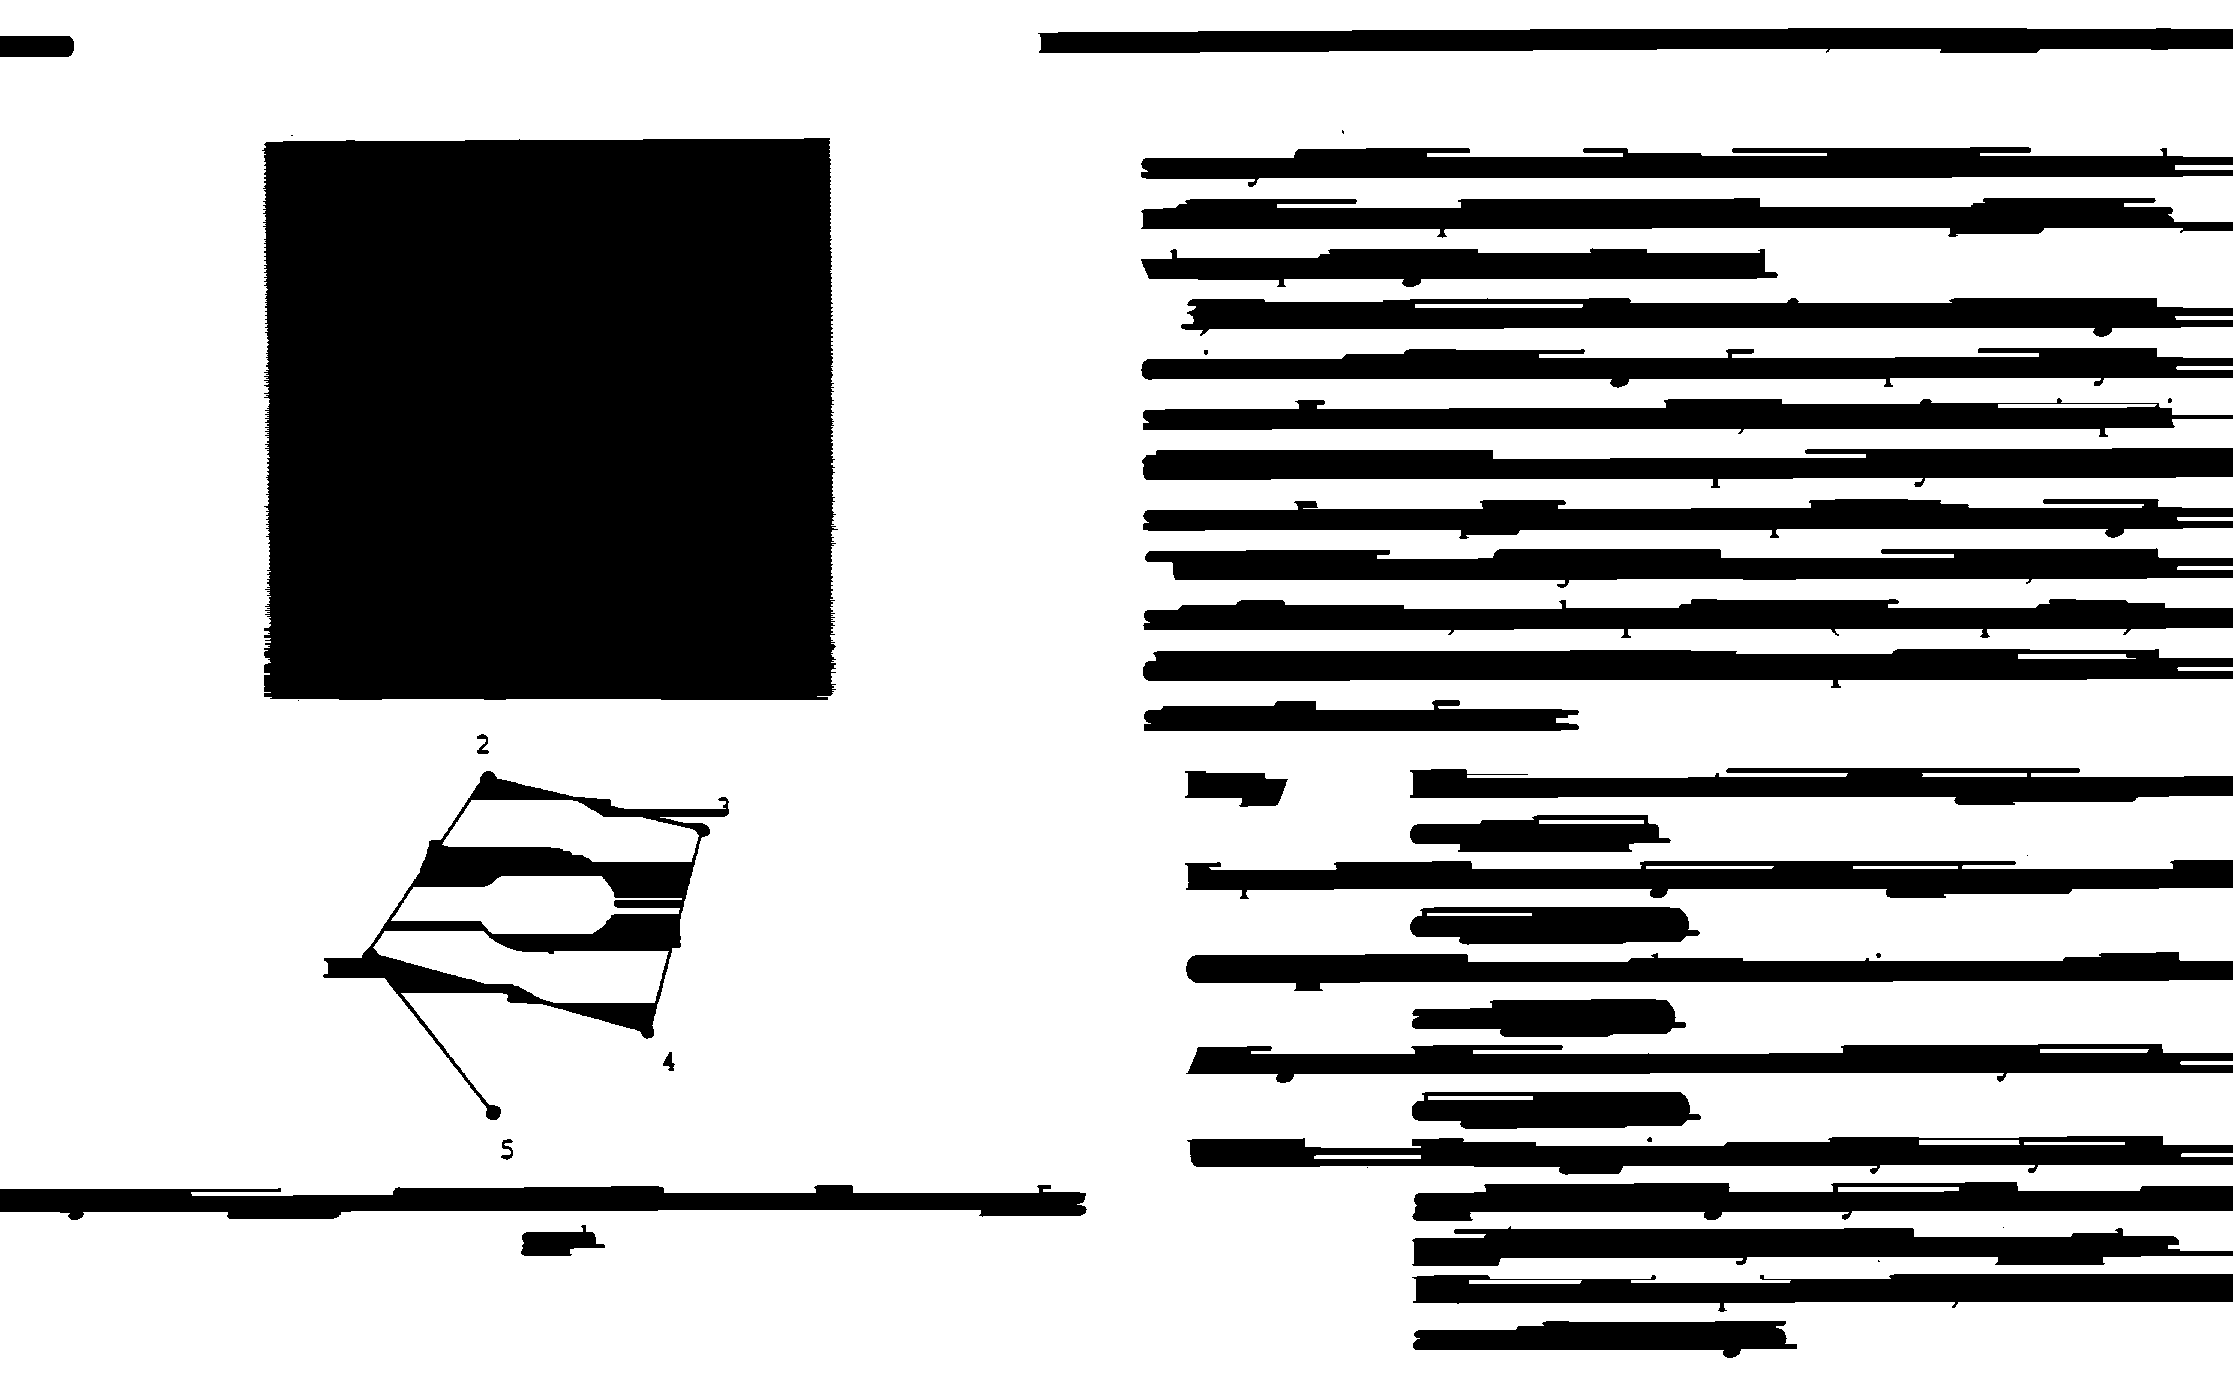
\includegraphics[width=.9\linewidth]{./img/step2.png}
\caption{Resultado do primeiro fechamento, \emph{kernel} \((1,100)\).}
\end{figure}

\begin{figure}[htbp]
\centering
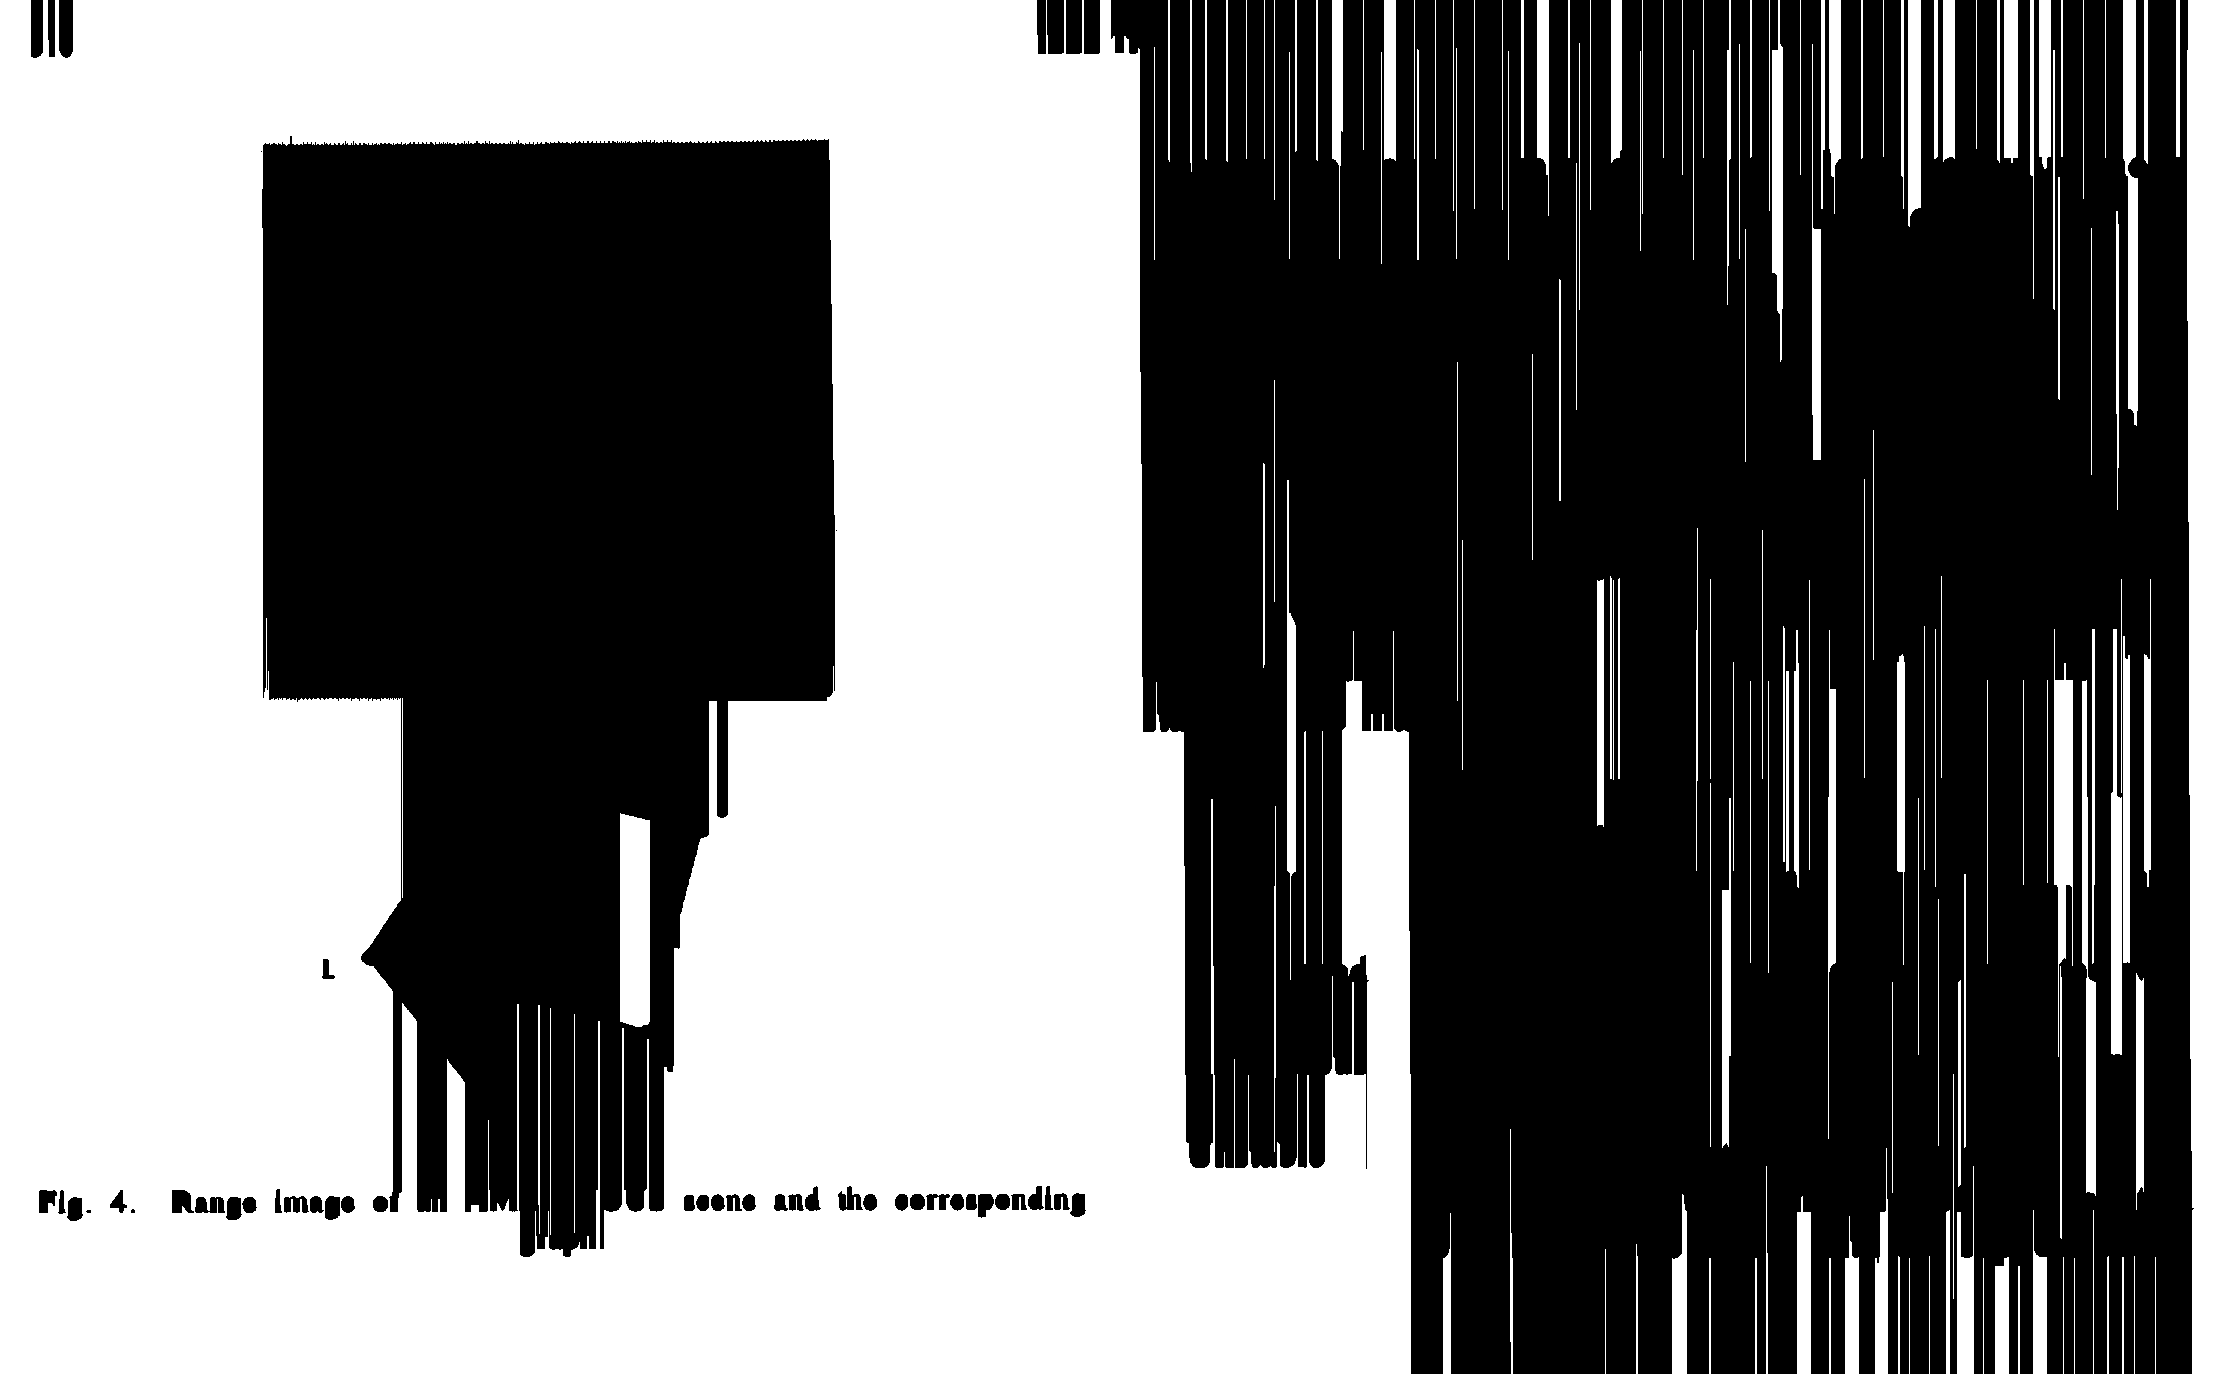
\includegraphics[width=.9\linewidth]{./img/step4.png}
\caption{Resultado do segundo fechamento, \emph{kernel} \((200,1)\).}
\end{figure}

Por fim, juntaremos ambas imagens geradas por meio de um operador lógico de \emph{and} e utilizamos a função \texttt{cv2.morphologyEx} com parâmetro \texttt{cv2.MORPH\_CLOSE} e um operador morfológico de dimensão \((1,30)\) para realizar o fechamento.
\begin{Code}
\begin{Verbatim}
\color{EFD}\textcolor[HTML]{a0522d}{img} \textcolor[HTML]{9370db}{=} cv2.\textcolor[HTML]{37474F}{\textbf{\textit{bitwise\_and}}}(img1, img2)

\textcolor[HTML]{a0522d}{kernel} \textcolor[HTML]{9370db}{=} np.\textcolor[HTML]{37474F}{\textbf{\textit{ones}}}((\textcolor[HTML]{29B6F6}{1}, \textcolor[HTML]{29B6F6}{30}), np.\textit{uint8})
\textcolor[HTML]{a0522d}{img} \textcolor[HTML]{9370db}{=} cv2.\textcolor[HTML]{37474F}{\textbf{\textit{morphologyEx}}}(img, cv2.\textcolor[HTML]{008b8b}{\textit{MORPH\_CLOSE}}, kernel)
\end{Verbatim}
\end{Code}

\begin{figure}[htbp]
\centering
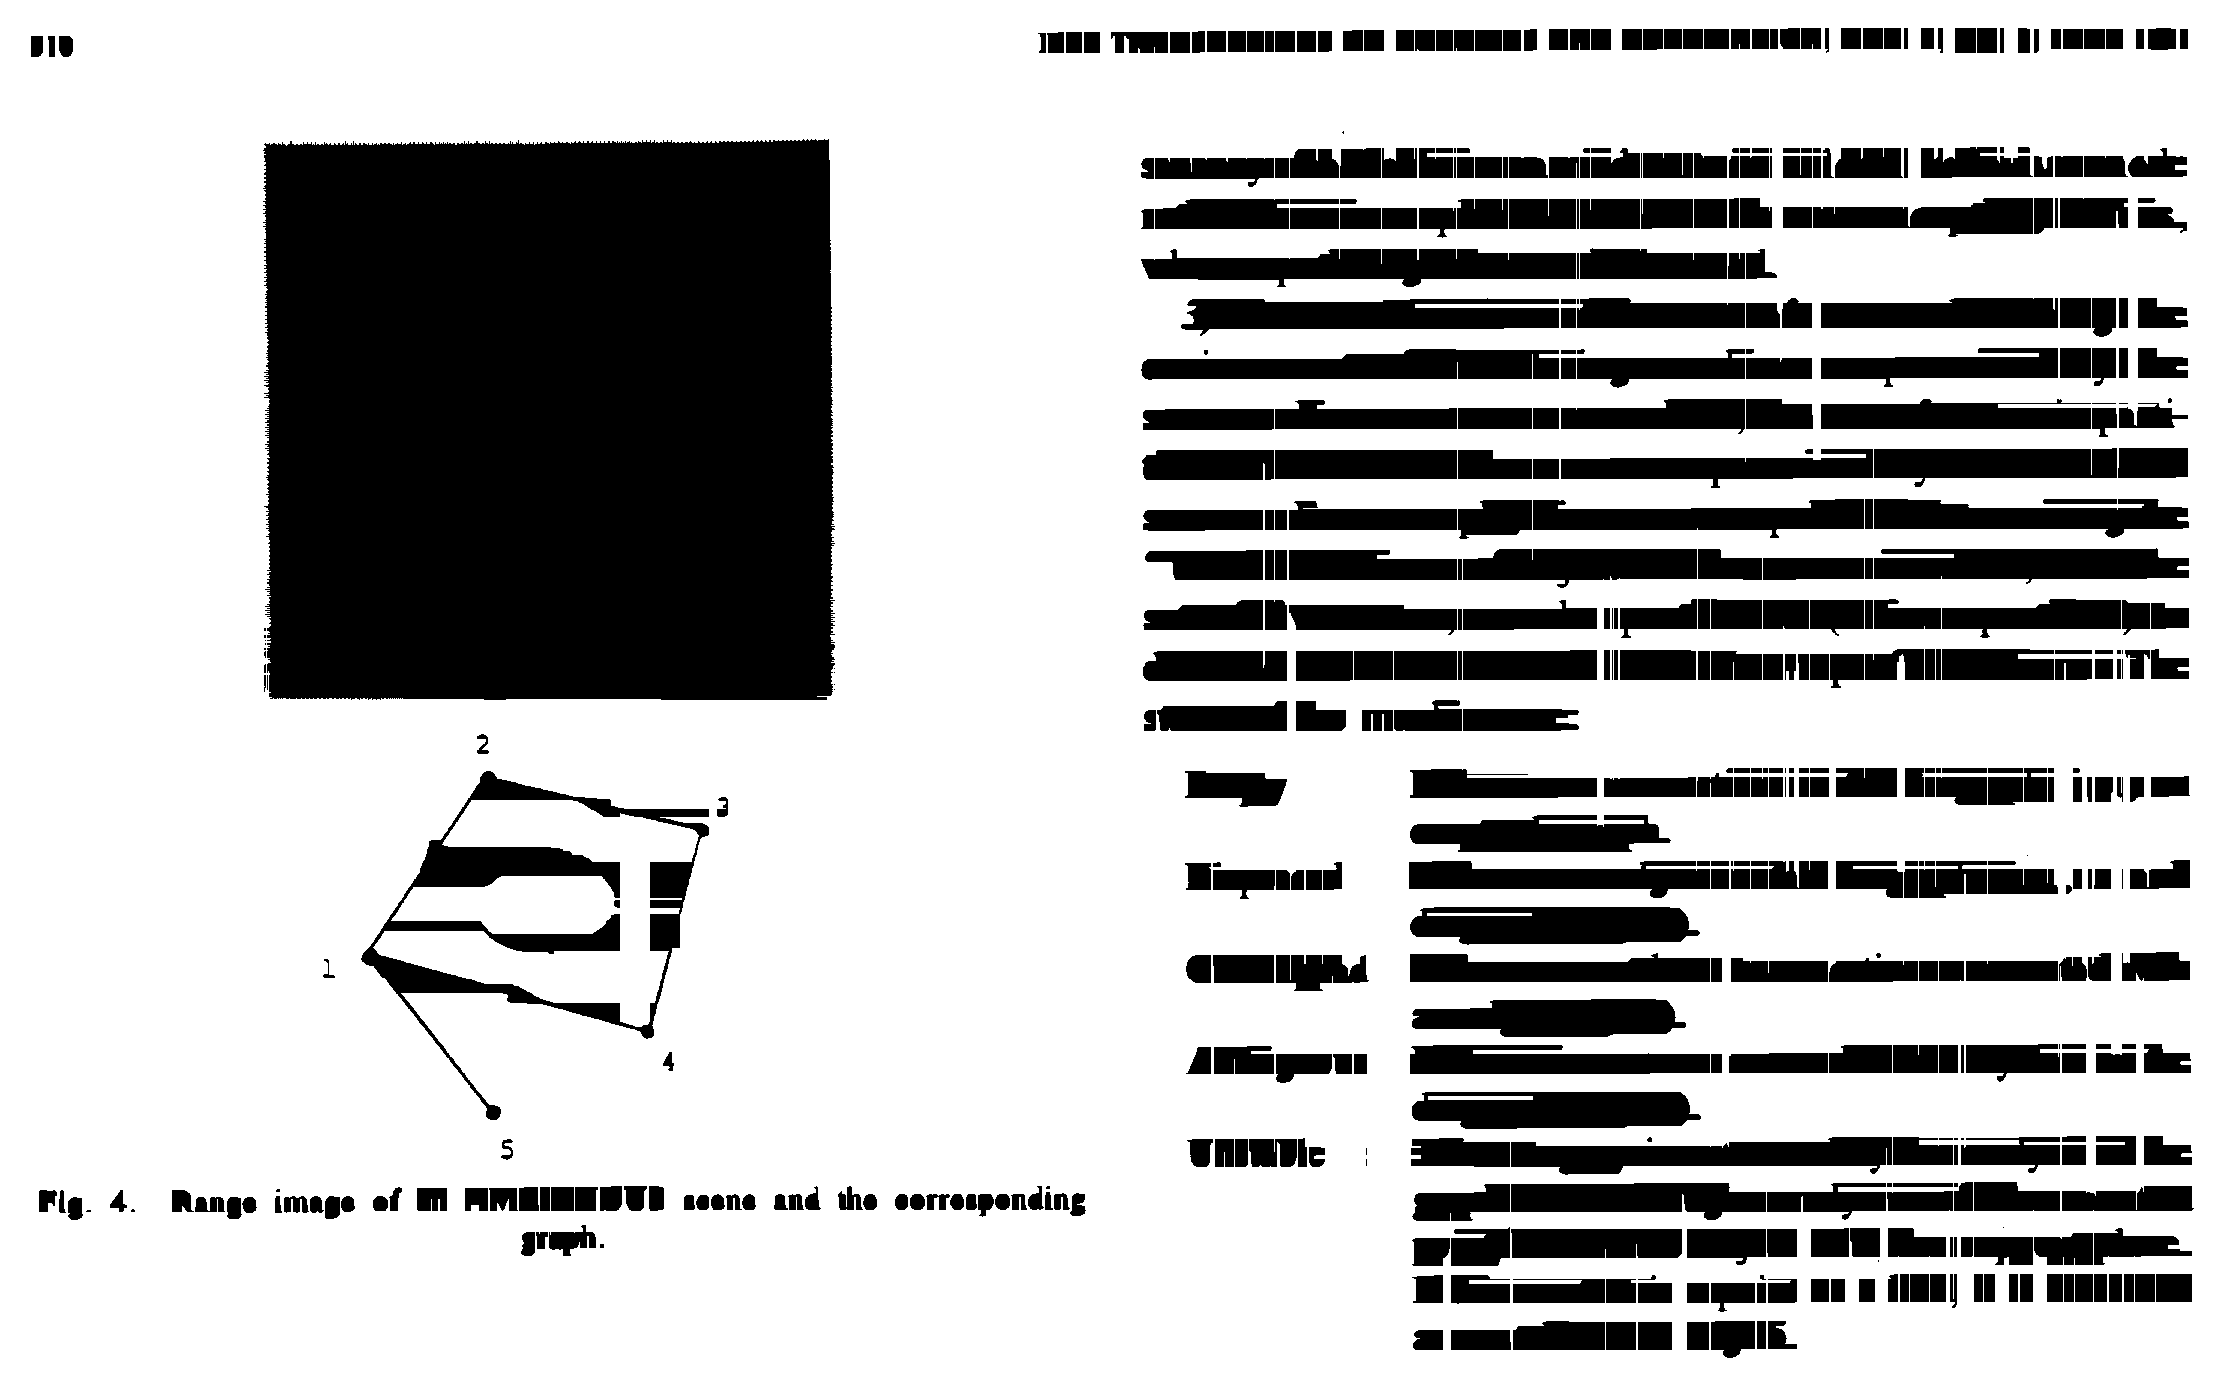
\includegraphics[width=.9\linewidth]{./img/step5.png}
\caption{Resultado da intersecção entre as imagens produzidas nos passos anteriores.}
\end{figure}

\begin{figure}[htbp]
\centering
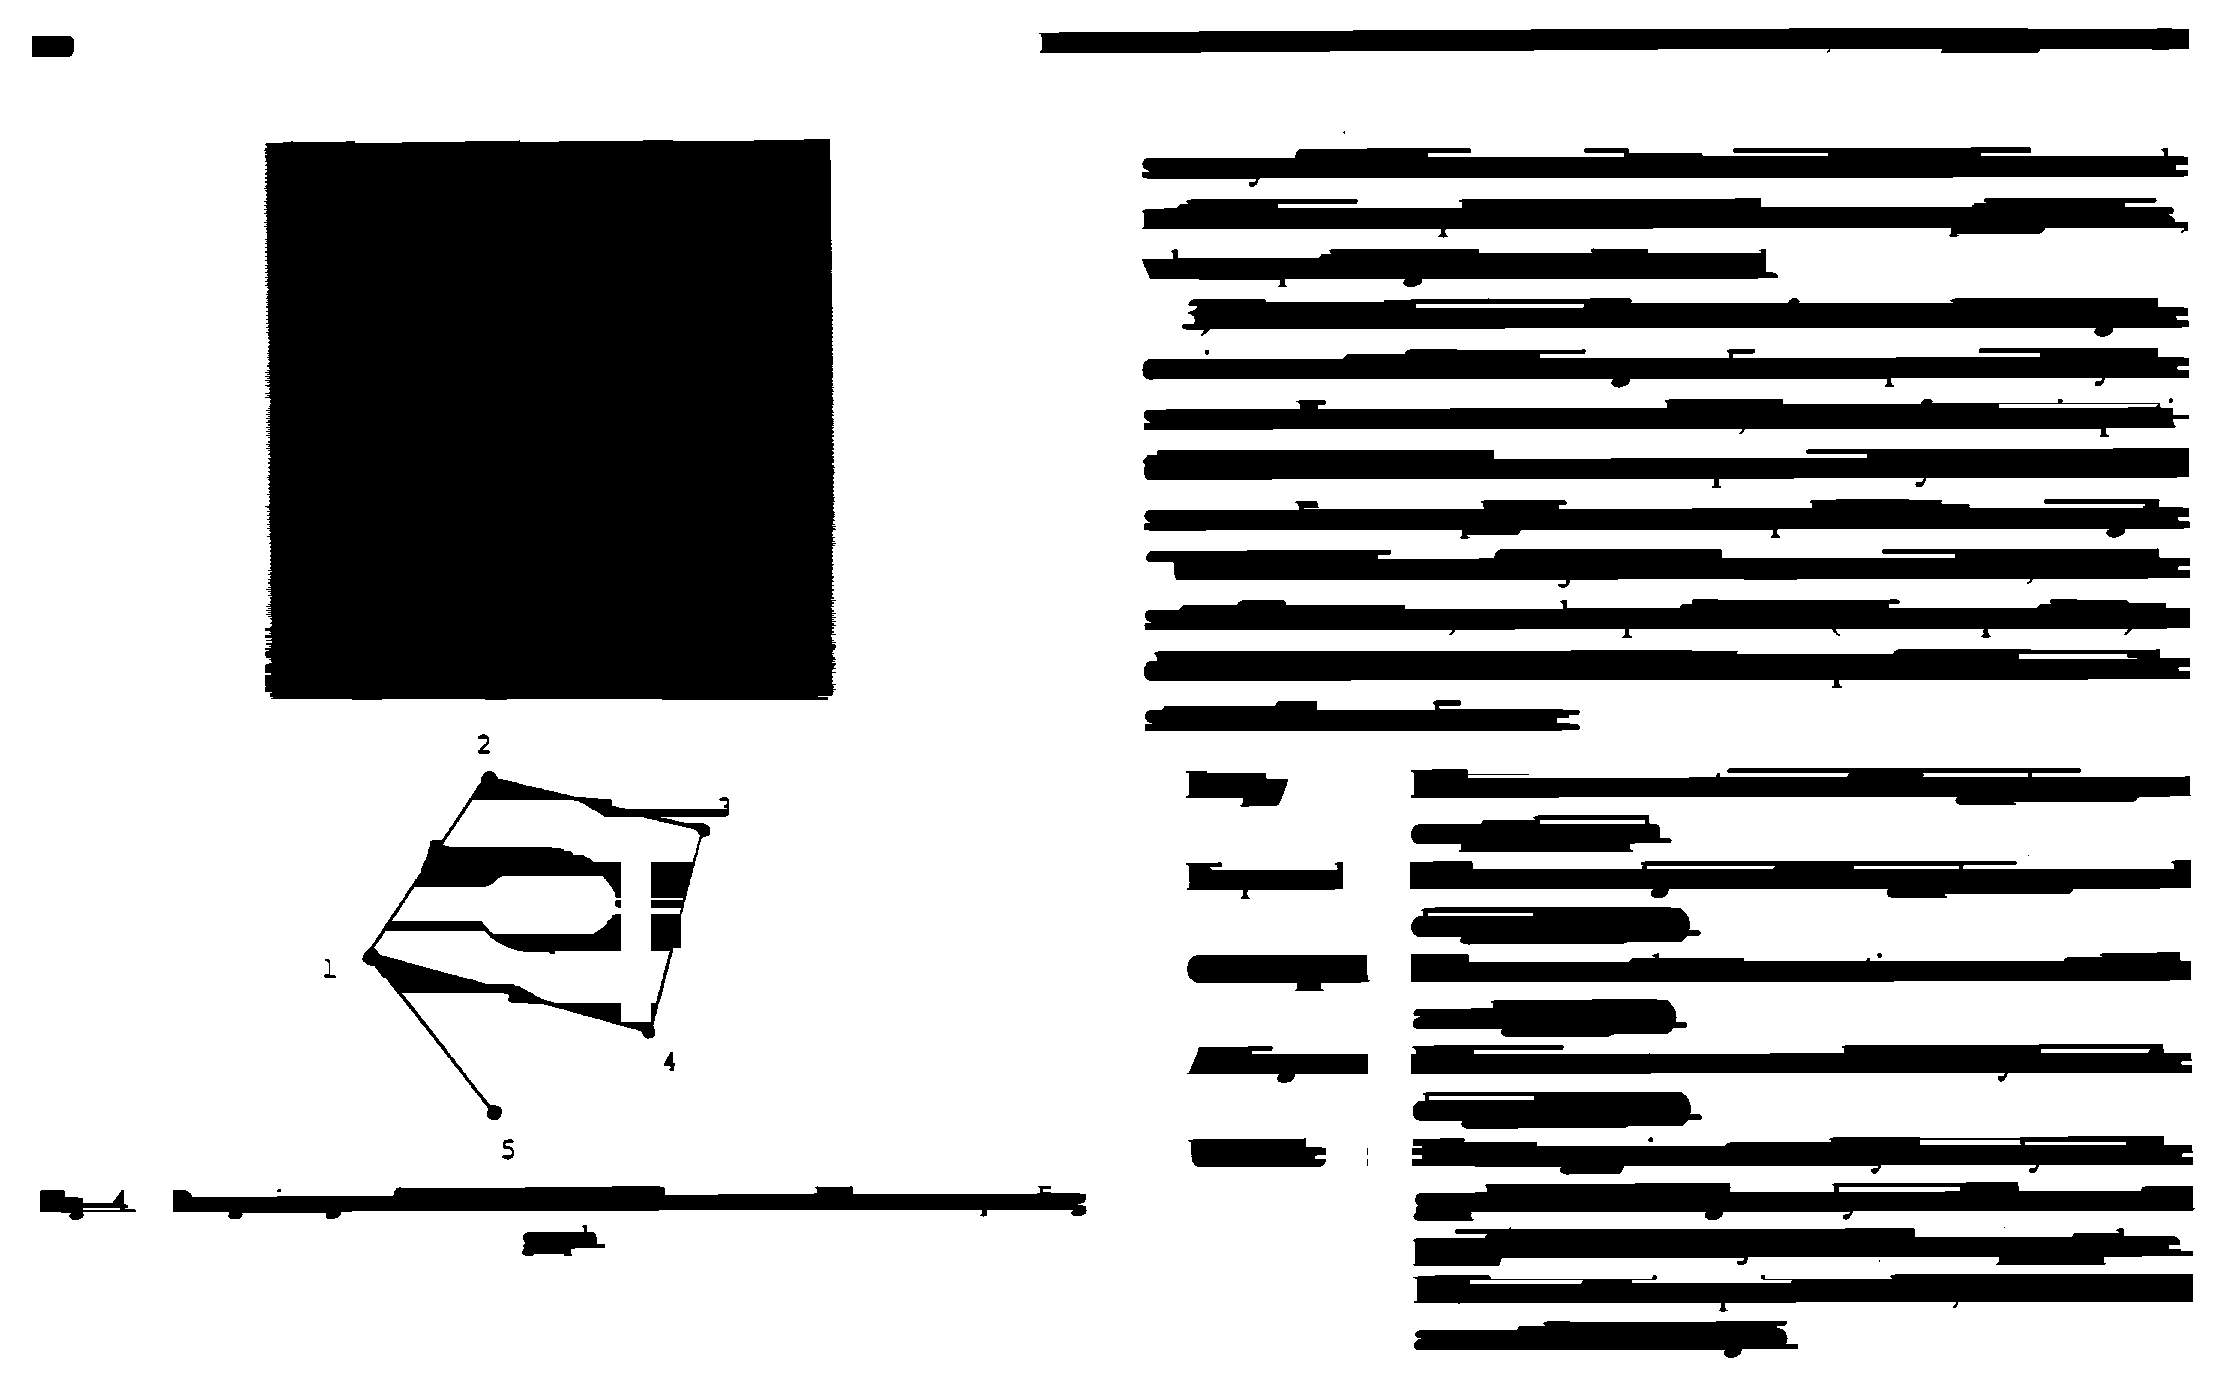
\includegraphics[width=.9\linewidth]{./img/step6.png}
\caption{Resultado da operação de fechamento, \emph{kernel} \((1,30)\).}
\end{figure}

Assim, ao final, possuímos componentes conexas que muito se assemelham à região que a linha de texto ocupava, com exceção das imagens.
Precisamos, por tanto, analisar mais a fundo as propriedades destas regiões para determinar quais são textos e quais não o são.

\section*{Componentes conexas}
\label{sec:orgc1976ad}
O primeiro passo é detectar as componentes conexas que aparecem na image.
Para tal, utilizamores a função \texttt{cv2.connectedComponentsWithStats}.
Esta recebe a imagem sob a qual aplicaremos o algoritmo de detecção de componentes conexas, bem como o tipo de vizinhança (utilizaremos \(8\)).
Demais parâmetros são utilizados para indicar onde esta função irá colocar os resultados, mas neste caso, iremos recebe-los no retorno desta e os mantemos como \texttt{None}.
\begin{Code}
\begin{Verbatim}
\color{EFD}\textcolor[HTML]{a0522d}{nlabels}, \textcolor[HTML]{a0522d}{\_}, \textcolor[HTML]{a0522d}{stats}, \textcolor[HTML]{a0522d}{\_} \textcolor[HTML]{9370db}{=}
    cv2.\textcolor[HTML]{37474F}{\textbf{\textit{connectedComponentsWithStats}}}(
        img, \textcolor[HTML]{483d8b}{None}, \textcolor[HTML]{483d8b}{None}, \textcolor[HTML]{483d8b}{None}, \textcolor[HTML]{29B6F6}{8}, cv2.\textcolor[HTML]{008b8b}{\textit{CV\_32S}}
    )
\end{Verbatim}
\end{Code}

Assim, possuímos uma lista de dados sobre as componentes (lista \texttt{stats}) e a quantidade destas (inteiro \texttt{nlabels}).
A variável \texttt{stats} possui \texttt{nlabels} elementos com as informações de cada componente conexo.
Estas incluem: as coordenadas do canto superior esquerdo do retângulo ao redor da componente e as dimensões de tal retângulo, bem como outras informações que não nos serão úteis nesse momento.

Com tais informações, podemos remover janelas da imagem original que correspondem a tais componentes conexas e, a partir destas janelas, analisar certas estatísticas que nos permitirão determinar se o conteúdo delas é ou não texto.

\begin{Code}
\begin{Verbatim}
\color{EFD}\textcolor[HTML]{b22222}{\# read original image}
\textcolor[HTML]{a0522d}{img} \textcolor[HTML]{9370db}{=} cv2.\textcolor[HTML]{37474F}{\textbf{\textit{imread}}}(\textcolor[HTML]{8b2252}{"bitmap.pbm"},
                 cv2.\textcolor[HTML]{008b8b}{\textit{IMREAD\_UNCHANGED}})
\textcolor[HTML]{a0522d}{text} \textcolor[HTML]{9370db}{=} [] \textcolor[HTML]{b22222}{\# data about the windows}
\textcolor[HTML]{9370db}{for} \textcolor[HTML]{a0522d}{i} \textcolor[HTML]{9370db}{in} \textcolor[HTML]{483d8b}{\textbf{range}}(nlabels):
    \textcolor[HTML]{a0522d}{x}, \textcolor[HTML]{a0522d}{y}, \textcolor[HTML]{a0522d}{w}, \textcolor[HTML]{a0522d}{h} \textcolor[HTML]{9370db}{=} stats[i][:\textcolor[HTML]{29B6F6}{4}]
    \textcolor[HTML]{a0522d}{crop} \textcolor[HTML]{9370db}{=} img[y : y \textcolor[HTML]{9370db}{+} h, x : x \textcolor[HTML]{9370db}{+} w]
    text.\textcolor[HTML]{37474F}{\textbf{\textit{append}}}([x, y, w, h, b])
    text[\textcolor[HTML]{9370db}{-}\textcolor[HTML]{29B6F6}{1}].\textcolor[HTML]{37474F}{\textbf{\textit{append}}}(\textcolor[HTML]{37474F}{\textbf{percentage}}(crop))
    text[\textcolor[HTML]{9370db}{-}\textcolor[HTML]{29B6F6}{1}].\textcolor[HTML]{37474F}{\textbf{\textit{append}}}(\textcolor[HTML]{37474F}{\textbf{v\_transitions}}(crop))
    text[\textcolor[HTML]{9370db}{-}\textcolor[HTML]{29B6F6}{1}].\textcolor[HTML]{37474F}{\textbf{\textit{append}}}(\textcolor[HTML]{37474F}{\textbf{h\_transitions}}(crop))
\end{Verbatim}
\end{Code}

A primeira estatística interessante é o percentual de pixels pretos em cada janela.
Calculamo-no utilizando a nossa função \texttt{percentage}.
\begin{Code}
\begin{Verbatim}
\color{EFD}\textcolor[HTML]{9370db}{def} \textcolor[HTML]{0000ff}{percentage}(\textcolor[HTML]{a0522d}{img}) -> \textcolor[HTML]{483d8b}{float}:
    \textcolor[HTML]{a0522d}{black} \textcolor[HTML]{9370db}{=} np.\textcolor[HTML]{37474F}{\textbf{\textit{count\_nonzero}}}(img \textcolor[HTML]{9370db}{==} \textcolor[HTML]{29B6F6}{0})
    \textcolor[HTML]{a0522d}{total} \textcolor[HTML]{9370db}{=} img.\textit{shape}[\textcolor[HTML]{29B6F6}{0}] \textcolor[HTML]{9370db}{*} img.\textit{shape}[\textcolor[HTML]{29B6F6}{1}]
    \textcolor[HTML]{9370db}{return} \textcolor[HTML]{483d8b}{\textbf{round}}(black \textcolor[HTML]{9370db}{/} total, \textcolor[HTML]{29B6F6}{2})
\end{Verbatim}
\end{Code}
Observamos que a maioria das janelas possuíam

Outro dado interessante é a quantidade de transições verticais ou horizontais de pixels brancos para pretos em relação ao número total de pixels pretos.
Podemos encontrar tal dado com as nossas funções \texttt{h\_transitions} e \texttt{v\_transitions}.
Por questões de espaço, aqui só reproduziremos uma delas, mas a outra é similar.

\begin{Code}
\begin{Verbatim}
\color{EFD}\textcolor[HTML]{9370db}{def} \textcolor[HTML]{0000ff}{h\_transitions}(\textcolor[HTML]{a0522d}{img}) -> \textcolor[HTML]{483d8b}{int}:
    \textcolor[HTML]{a0522d}{transitions} \textcolor[HTML]{9370db}{=} \textcolor[HTML]{29B6F6}{0}
    \textcolor[HTML]{9370db}{for} \textcolor[HTML]{a0522d}{i} \textcolor[HTML]{9370db}{in} \textcolor[HTML]{483d8b}{\textbf{range}}(img.\textit{shape}[\textcolor[HTML]{29B6F6}{0}] \textcolor[HTML]{9370db}{-} \textcolor[HTML]{29B6F6}{1}):
        \textcolor[HTML]{9370db}{for} \textcolor[HTML]{a0522d}{j} \textcolor[HTML]{9370db}{in} \textcolor[HTML]{483d8b}{\textbf{range}}(img.\textit{shape}[\textcolor[HTML]{29B6F6}{1}]):
            \textcolor[HTML]{9370db}{if} (img[i][j] \textcolor[HTML]{9370db}{==} \textcolor[HTML]{29B6F6}{0} \textcolor[HTML]{9370db}{and}
                img[i \textcolor[HTML]{9370db}{+} \textcolor[HTML]{29B6F6}{1}][j] \textcolor[HTML]{9370db}{==} \textcolor[HTML]{29B6F6}{255}):
                \textcolor[HTML]{a0522d}{transitions} \textcolor[HTML]{9370db}{+=} \textcolor[HTML]{29B6F6}{1}
    \textcolor[HTML]{a0522d}{black} \textcolor[HTML]{9370db}{=} np.\textcolor[HTML]{37474F}{\textbf{\textit{count\_nonzero}}}(img \textcolor[HTML]{9370db}{==} \textcolor[HTML]{29B6F6}{0})
    \textcolor[HTML]{9370db}{if} black \textcolor[HTML]{9370db}{==} \textcolor[HTML]{29B6F6}{0}:
        \textcolor[HTML]{9370db}{return} \textcolor[HTML]{29B6F6}{0}
    \textcolor[HTML]{9370db}{return} \textcolor[HTML]{483d8b}{\textbf{round}}(transitions \textcolor[HTML]{9370db}{/} black, \textcolor[HTML]{29B6F6}{3})
\end{Verbatim}
\end{Code}

Com tais informações em mãos, determinamos que as componente que realmente representam texto são aquelas que possuem percentual de pixels pretos entre \(9\%\) e \(40\%\) e frequência de transições de pixels brancos para pretos entre \(9\%\) e \(40\%\).
Por fim, adicionamos uma retrição na altura da componente conexa em especial para eliminar a componente que envolve a imagem inteira.
\begin{Code}
\begin{Verbatim}
\color{EFD}\textcolor[HTML]{a0522d}{text} \textcolor[HTML]{9370db}{=} [
    comp
    \textcolor[HTML]{9370db}{for} \textcolor[HTML]{a0522d}{comp} \textcolor[HTML]{9370db}{in} text
    \textcolor[HTML]{9370db}{if} (
        \textcolor[HTML]{29B6F6}{20} \textcolor[HTML]{9370db}{<} comp[\textcolor[HTML]{29B6F6}{3}] \textcolor[HTML]{9370db}{<} \textcolor[HTML]{29B6F6}{50}
        \textcolor[HTML]{9370db}{and} \textcolor[HTML]{29B6F6}{0.09} \textcolor[HTML]{9370db}{<} comp[\textcolor[HTML]{29B6F6}{5}] \textcolor[HTML]{9370db}{<} \textcolor[HTML]{29B6F6}{0.4}
        \textcolor[HTML]{9370db}{and} \textcolor[HTML]{29B6F6}{0.09} \textcolor[HTML]{9370db}{<} comp[\textcolor[HTML]{29B6F6}{6}] \textcolor[HTML]{9370db}{<} \textcolor[HTML]{29B6F6}{0.4}
        \textcolor[HTML]{9370db}{and} \textcolor[HTML]{29B6F6}{0.09} \textcolor[HTML]{9370db}{<} comp[\textcolor[HTML]{29B6F6}{7}] \textcolor[HTML]{9370db}{<} \textcolor[HTML]{29B6F6}{0.4}
    )
]
\end{Verbatim}
\end{Code}

Por fim, nossa variável \texttt{text} possui as informações sobre cada \emph{bounding box} de cada linha.
Podemos desenha-las numa imagem \emph{RGB} com a cor verde para ilustrar.
\begin{Code}
\begin{Verbatim}
\color{EFD}\textcolor[HTML]{a0522d}{img} \textcolor[HTML]{9370db}{=} cv2.\textcolor[HTML]{37474F}{\textbf{\textit{cvtColor}}}(img, cv2.\textcolor[HTML]{008b8b}{\textit{COLOR\_GRAY2RGB}})
\textcolor[HTML]{9370db}{for} \textcolor[HTML]{a0522d}{line} \textcolor[HTML]{9370db}{in} text:
    \textcolor[HTML]{a0522d}{x}, \textcolor[HTML]{a0522d}{y}, \textcolor[HTML]{a0522d}{w}, \textcolor[HTML]{a0522d}{h} \textcolor[HTML]{9370db}{=} line[:\textcolor[HTML]{29B6F6}{4}]
    \textcolor[HTML]{a0522d}{img} \textcolor[HTML]{9370db}{=} cv2.\textcolor[HTML]{37474F}{\textbf{\textit{rectangle}}}(img, \textcolor[HTML]{b22222}{\# imagem}
                        (x, y), \textcolor[HTML]{b22222}{\# toplef}
                        (x \textcolor[HTML]{9370db}{+} w, y \textcolor[HTML]{9370db}{+} h),
                        (\textcolor[HTML]{29B6F6}{0}, \textcolor[HTML]{29B6F6}{255}, \textcolor[HTML]{29B6F6}{0}), \textcolor[HTML]{b22222}{\# color}
                        \textcolor[HTML]{29B6F6}{2}) \textcolor[HTML]{b22222}{\# thickness}
\end{Verbatim}
\end{Code}
\begin{figure}[htbp]
\centering
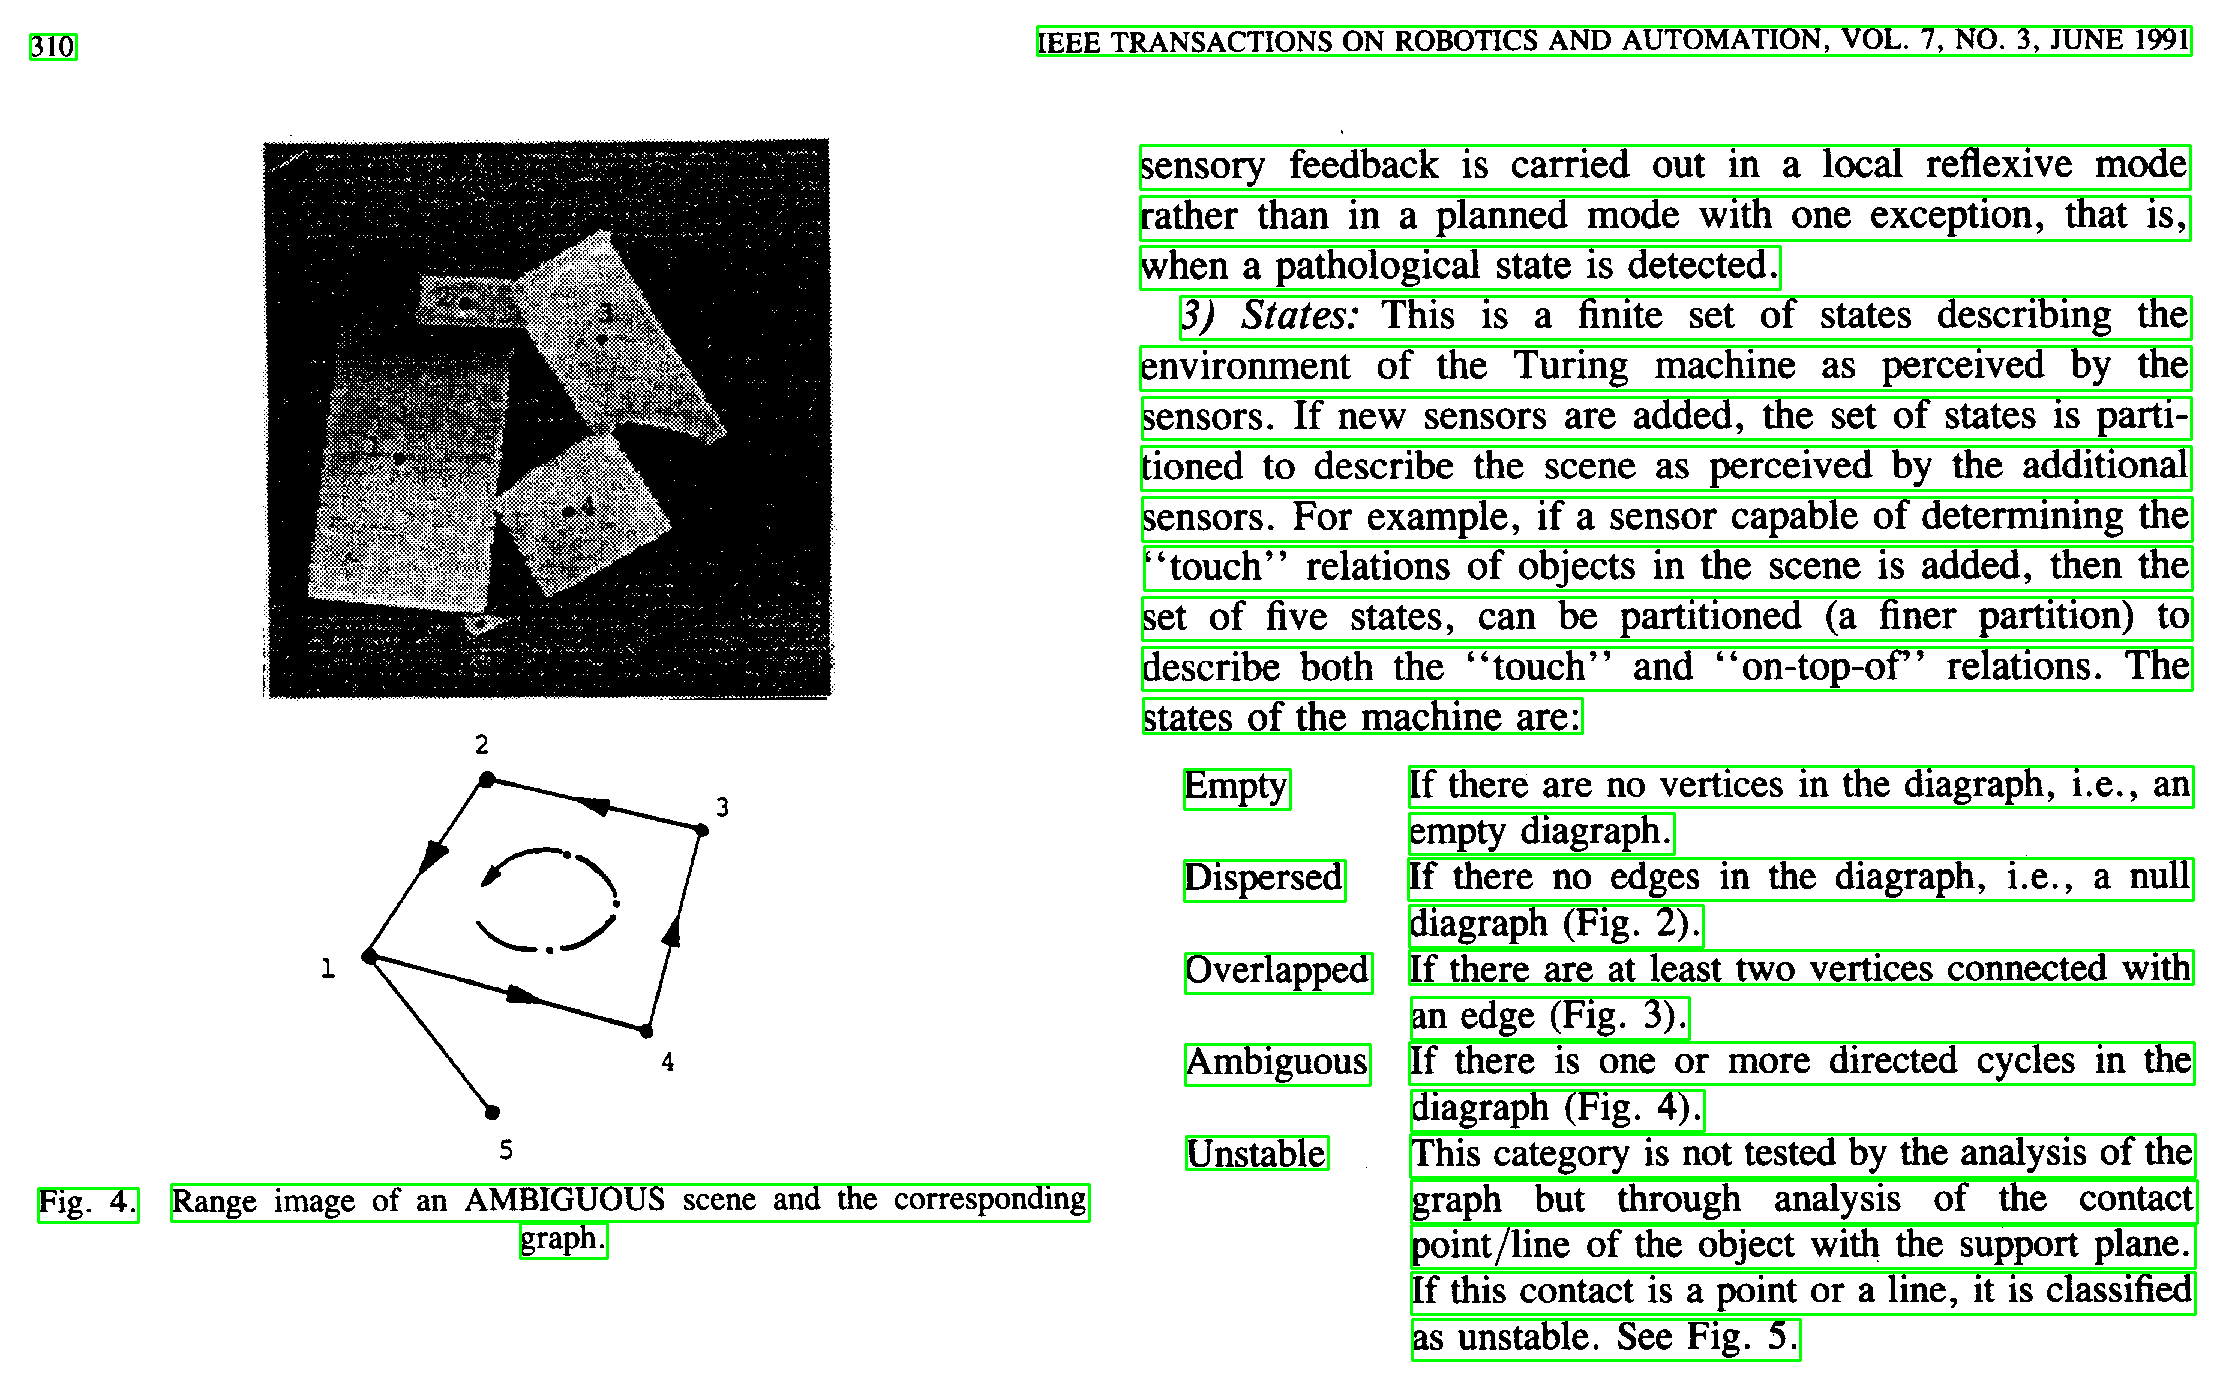
\includegraphics[width=.9\linewidth]{./img/lines.png}
\caption{Linhas detectadas cercadas por suas \emph{bounding boxes} em verde.}
\end{figure}

\section*{Palavras}
\label{sec:orgb1308cc}
Para detectar então cada palavra individualmente, podemos aplicar técnicas similares, mas agora apenas em janelas da imagem as quais sabemos ser texto.
Através de experimentação e se baseando na teoria, buscamos realizar a dilatação vertical e horizontal (elementos estruturantes \((1,10)\) e \((10,1)\)) das imagens e posterior fechamento (elemento estruturante \((1,3)\)).

\begin{figure}[htbp]
\centering
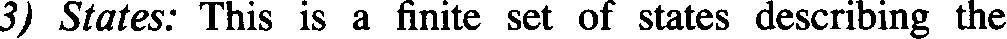
\includegraphics[width=.9\linewidth]{./img/line1.png}
\caption{Linha de texto inicial.}
\end{figure}

\begin{figure}[htbp]
\centering
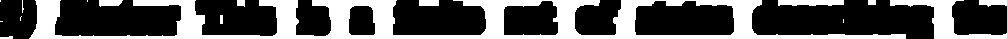
\includegraphics[width=.9\linewidth]{./img/line3.png}
\caption{Linha de texto dilatada com \emph{kernels} \((1,10)\) e \((10,1)\).}
\end{figure}

\begin{figure}[htbp]
\centering
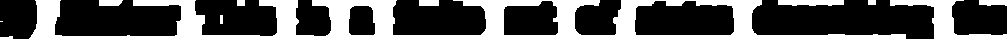
\includegraphics[width=.9\linewidth]{./img/line4.png}
\caption{Linha de texto após fechamento com \emph{kernel} \((1,3)\).}
\end{figure}

Assim, cada palavra se tornou um conexo ``borrão'', o que nos permite utilizar a mesma função de componentes conexas para determinas suas posições.
\begin{Code}
\begin{Verbatim}
\color{EFD}\textcolor[HTML]{9370db}{def} \textcolor[HTML]{0000ff}{detect\_words}(\textcolor[HTML]{a0522d}{img}):
    \textcolor[HTML]{a0522d}{kernel1} \textcolor[HTML]{9370db}{=} np.\textcolor[HTML]{37474F}{\textbf{\textit{ones}}}((\textcolor[HTML]{29B6F6}{1}, \textcolor[HTML]{29B6F6}{10}), np.\textit{uint8})
    \textcolor[HTML]{a0522d}{img} \textcolor[HTML]{9370db}{=} cv2.\textcolor[HTML]{37474F}{\textbf{\textit{dilate}}}(img, kernel1,
                     \textcolor[HTML]{483d8b}{\textbf{iterations}}\textcolor[HTML]{9370db}{=}\textcolor[HTML]{29B6F6}{1})

    \textcolor[HTML]{a0522d}{kernel2} \textcolor[HTML]{9370db}{=} np.\textcolor[HTML]{37474F}{\textbf{\textit{ones}}}((\textcolor[HTML]{29B6F6}{10}, \textcolor[HTML]{29B6F6}{1}), np.\textit{uint8})
    \textcolor[HTML]{a0522d}{img} \textcolor[HTML]{9370db}{=} cv2.\textcolor[HTML]{37474F}{\textbf{\textit{dilate}}}(img, kernel2,
                     \textcolor[HTML]{483d8b}{\textbf{iterations}}\textcolor[HTML]{9370db}{=}\textcolor[HTML]{29B6F6}{1})

    \textcolor[HTML]{a0522d}{kernel3} \textcolor[HTML]{9370db}{=} np.\textcolor[HTML]{37474F}{\textbf{\textit{ones}}}((\textcolor[HTML]{29B6F6}{1}, \textcolor[HTML]{29B6F6}{3}), np.\textit{uint8})
    \textcolor[HTML]{a0522d}{img} \textcolor[HTML]{9370db}{=} cv2.\textcolor[HTML]{37474F}{\textbf{\textit{morphologyEx}}}(img,
                           cv2.\textcolor[HTML]{008b8b}{\textit{MORPH\_CLOSE}},
                           kernel3)

    \textcolor[HTML]{9370db}{return} (
        cv2.\textcolor[HTML]{37474F}{\textbf{\textit{connectedComponentsWithStats}}}
            (img,\textcolor[HTML]{483d8b}{None},\textcolor[HTML]{483d8b}{None},\textcolor[HTML]{483d8b}{None},\textcolor[HTML]{29B6F6}{8},cv2.\textcolor[HTML]{008b8b}{\textit{CV\_32S}})
    )
\end{Verbatim}
\end{Code}

Por fim, podemos usar as \emph{bounding boxes} azuis para marcar as palavras e repetirmos o processo para cada linha.
Perceba que, as vezes, nosso algoritmo interpreta sequências como \texttt{(Fig.} como uma palavra.

\begin{figure}[htbp]
\centering
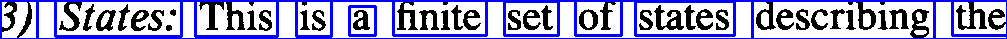
\includegraphics[width=.9\linewidth]{./img/line5.png}
\caption{Linha com as palavras marcadas em \emph{bouding boxes} azuis.}
\end{figure}

\section*{Conclusão}
\label{sec:org43673dc}
Neste trabalho, fomos capazes de aplicar os operadores morfológicos e, com isso, detectar \(35\) linhas de texto e \(241\) palavras.
\begin{figure}[htbp]
\centering
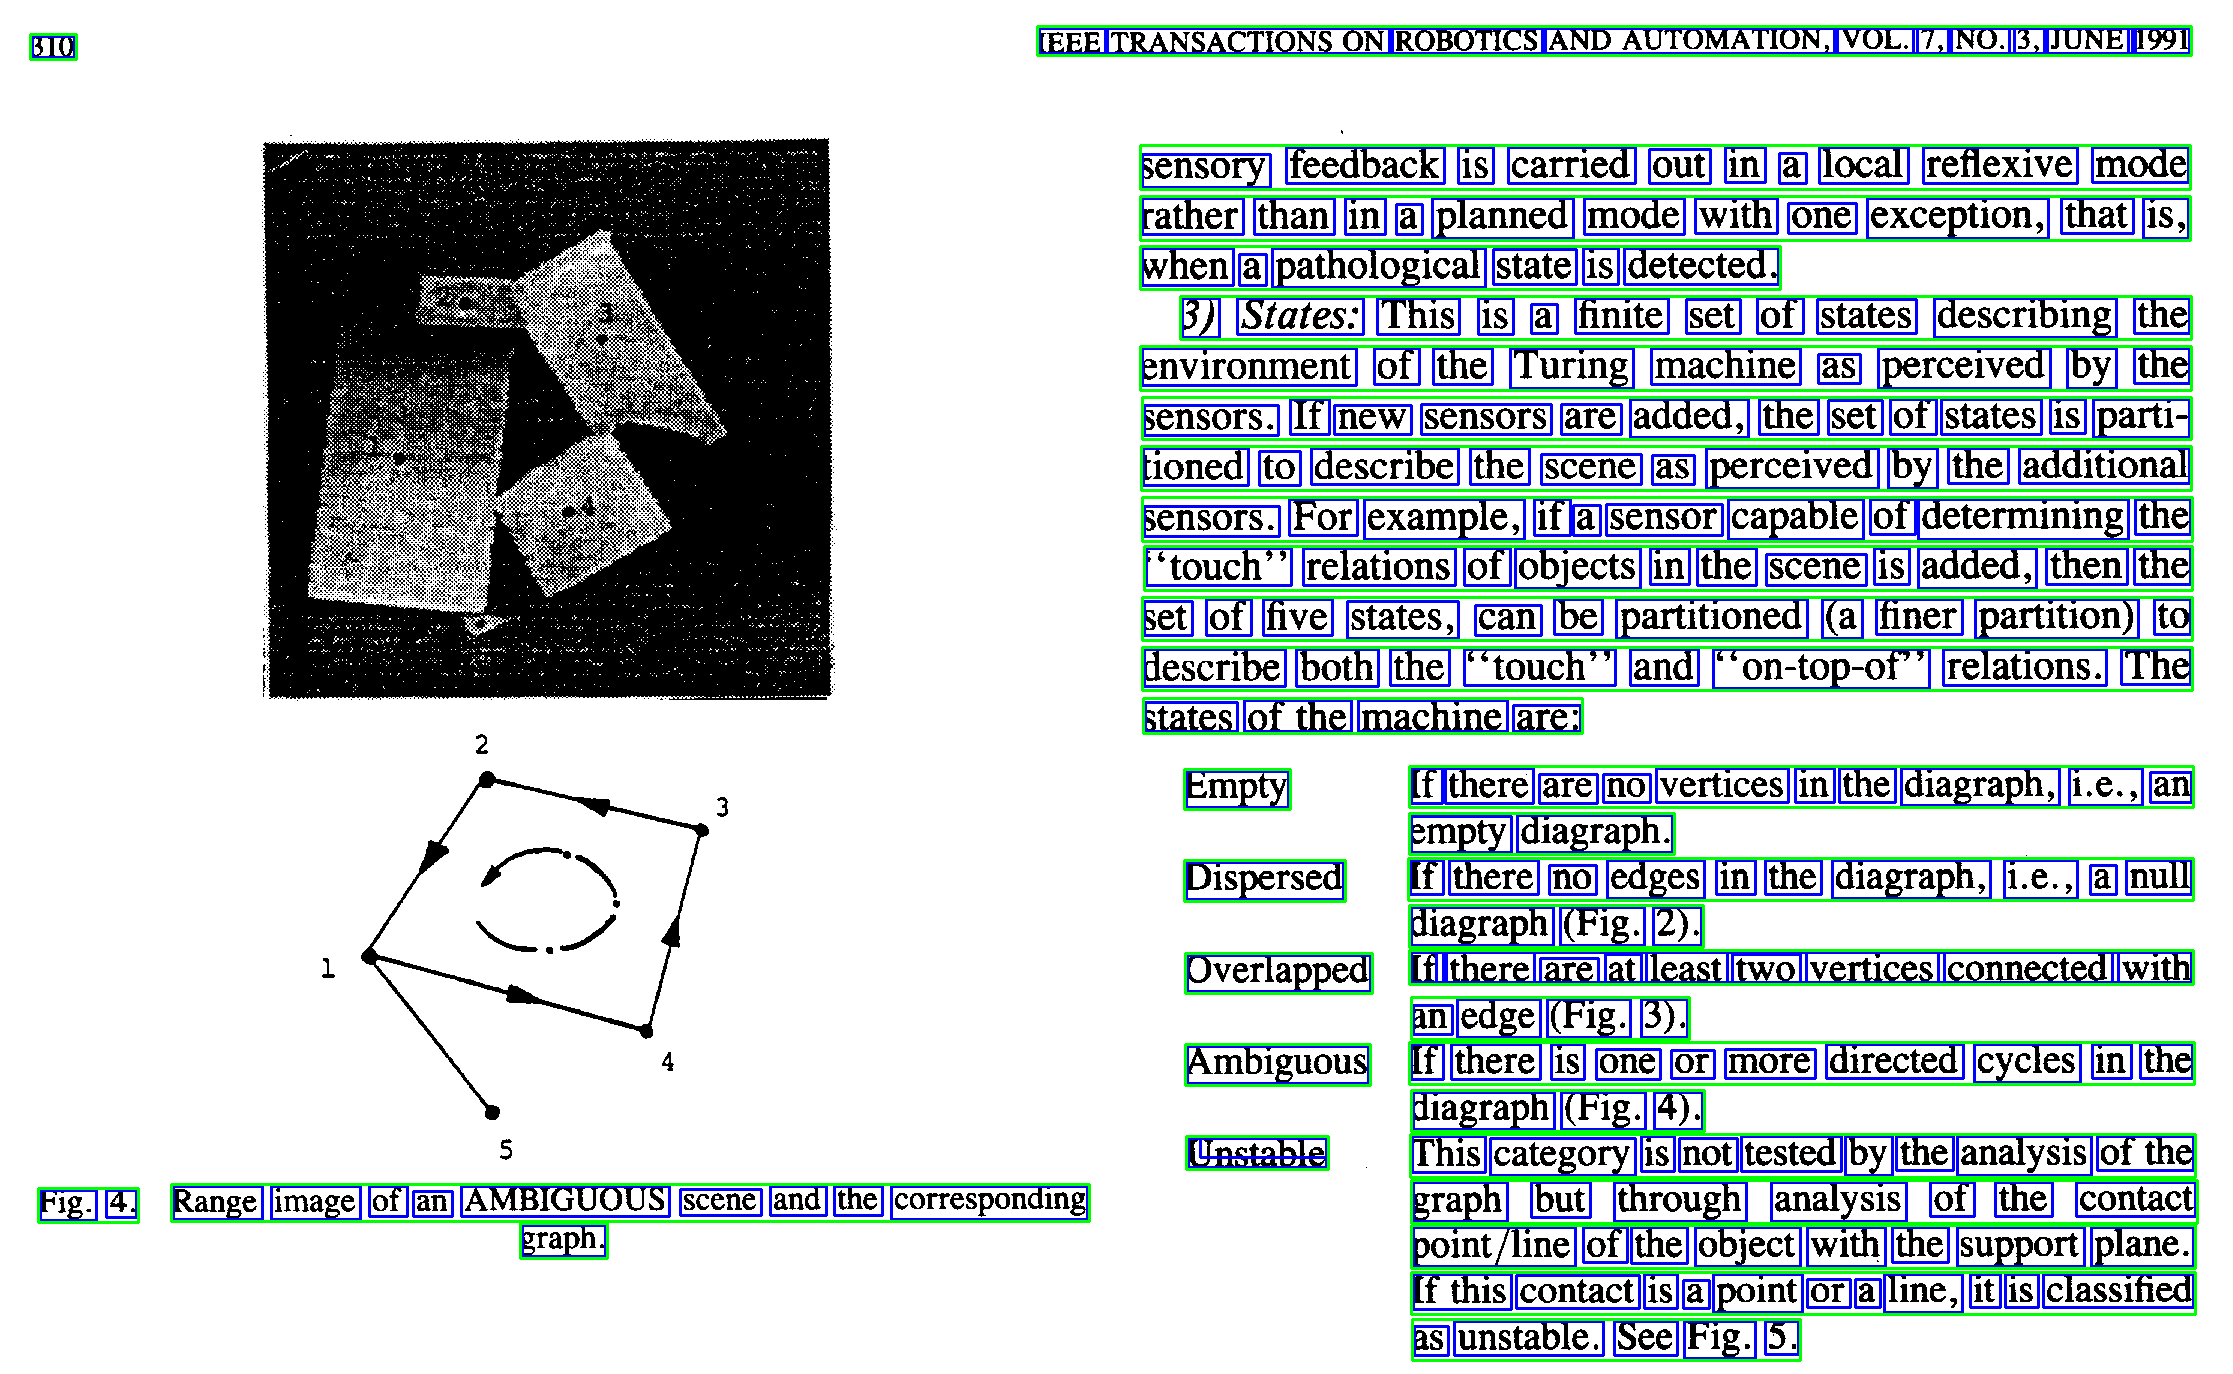
\includegraphics[width=.9\linewidth]{./img/out.png}
\caption{Imagem final. Linhas estão marcadas por caixas verdes e palavras por caixas azuis.}
\end{figure}

Como trabalhos futuros, ressaltamos a possibilidade de utilizar técnicas de clusterização para determinar as condições que caracterizam texto, como fizemos manualmente aqui. Assim seríamos capazes de processar textos mais diversos.
Além disso, baseado nas propriedades de componentes conexos de cada caractere, como a quantidade de buracos, pode ser feita a detecção de cada um deles e transcrição para texto.
\end{document}